%!TEX root = ../main.tex
\documentclass[../main.tex]{subfiles}
\begin{document}
\subsection{Additional Tables and Figures} \label{app:tables_and_figures}
\subsubsection{Correlation Heatmap of Task Choices}
\begin{figure}[!htbp]
	\centering
	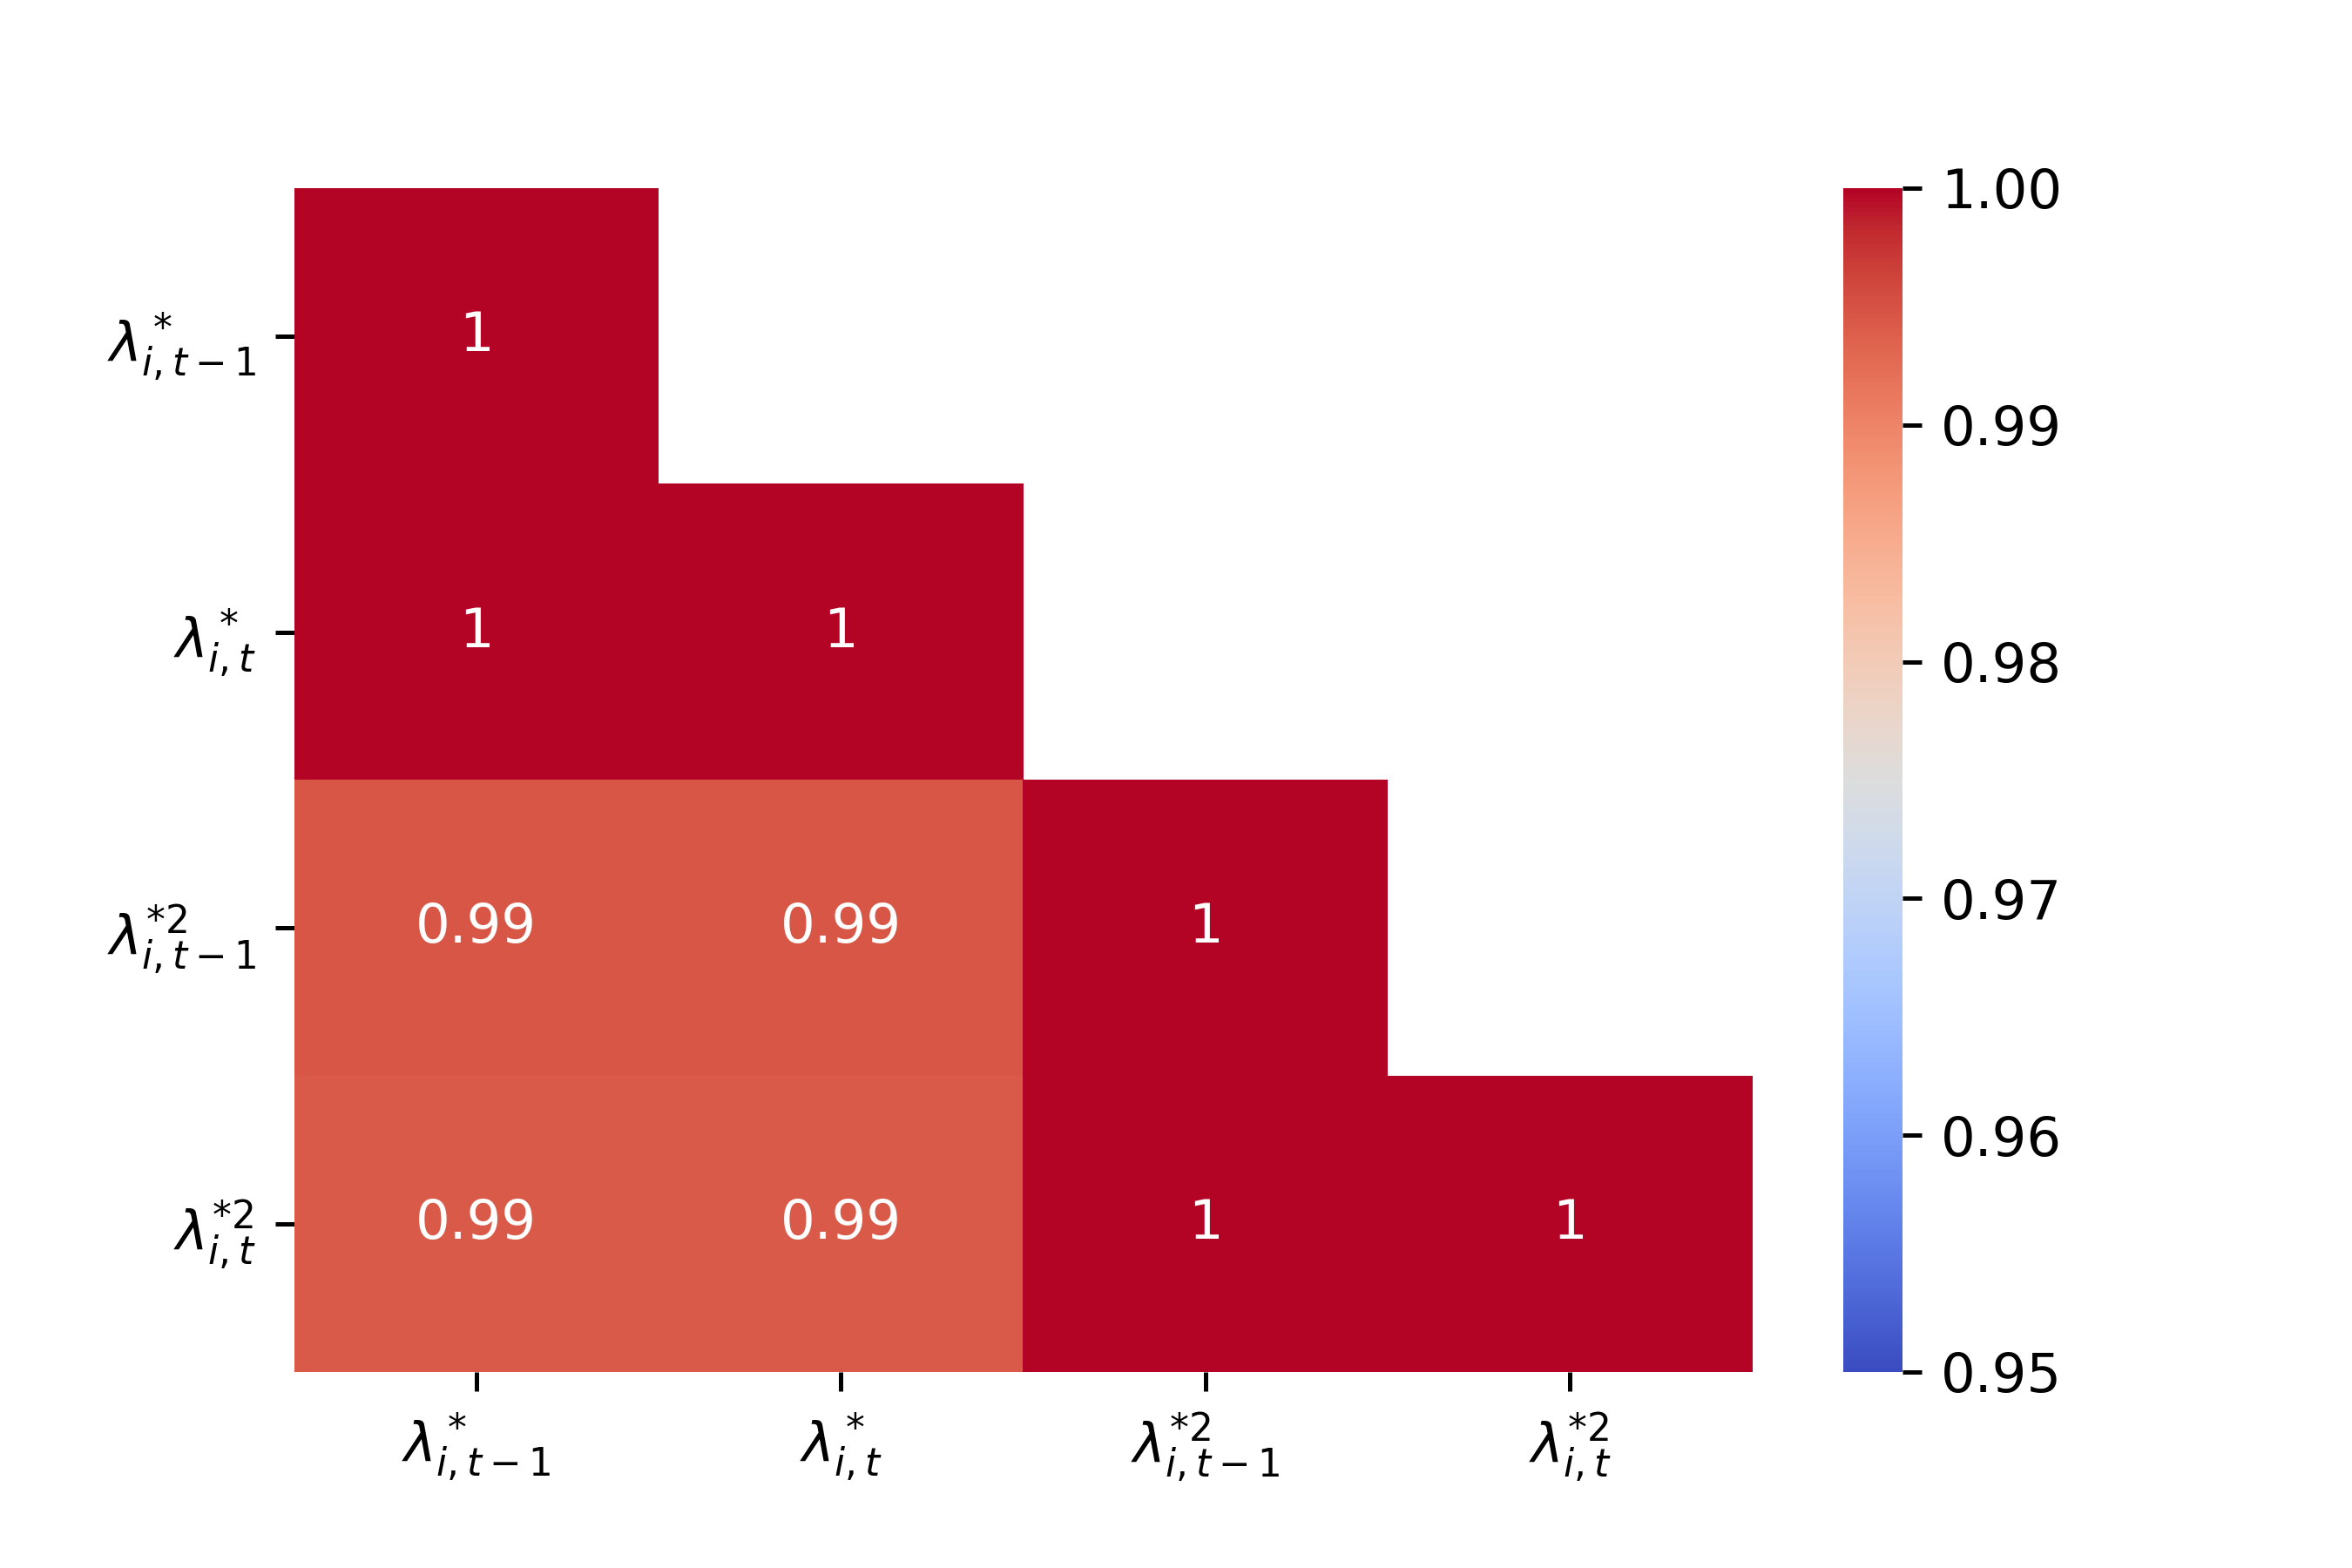
\includegraphics[scale=0.7]{./FIG/corr_heatmap.png} 
	\caption{Heatmap of correlation coefficients of task choices in periods $t-1$ and $t$ of the base period as well as their squared values. Notice that the scale is compressed and only covers values between 0.95 and 1.0 to make the small differences visible.}
	\label{fig:corr_heatmap}
\end{figure}

\FloatBarrier
\subsubsection{Estimation Results in Base Period}
%%%%%%%%%%%%%%%%%%%%%%%%%%%%%%%%%%%%% Table 1 %%%%%%%%%%%%%%%%%
\begin{table}[!htbp]
\begin{center}
\begin{tabular}{lclc}
\toprule
\textbf{Dep. Variable:}    & $\Delta w_{i,t}$ & \textbf{  R-squared (uncentered):}      &     0.999   \\
\textbf{No. Observations:} &       100        & \textbf{  Adj. R-squared (uncentered):} &     0.999   \\
\textbf{F-statistic:}      &  5.720e+04      & \textbf{  Prob (F-statistic):}          & 4.87e-151   \\
\bottomrule
\end{tabular}
\begin{tabular}{lcccccc}
                  & \textbf{coef} & \textbf{std err} & \textbf{t} & \textbf{P$> |$t$|$} & \textbf{[0.025} & \textbf{0.975]}  \\
\midrule
\textbf{$\lambda_{i, t-1}^{*}$}   &       -0.4989  &        0.002     &   -240.382  &         0.000        &        -0.503    &        -0.495     \\
\textbf{$\lambda_{i, t-1}^{*2}$} &        1.0001  &        0.004     &    278.381  &         0.000        &         0.993   &         1.007    \\
\bottomrule
\end{tabular}

\end{center}
\caption{Results of an OLS estimation of wage changes in the base period on both, $\lambda_{i, t-1}^{*}$ and $\lambda_{i, t-1}^{*2}$. This estimation result is from one of the $M = 1000$ simulated datasets used in the Monte Carlo estimation. Regressors do not include a constant because the true model intersects the point of origin due to the normalization of $w_{i,j=1,t} = 0$.}
\label{tab:base_period_regression_rlst_t-1}
\end{table}
%%%%%%%%%%%%%%%%%%%%%%%%%%%%%%%%%%%%% Table 2 %%%%%%%%%%%%%%%%%
\begin{table}[!htbp]
\begin{center}
\begin{tabular}{lclc}
\toprule
\textbf{Dep. Variable:}    & $\Delta w_{i,t}$ & \textbf{  R-squared (uncentered):}      &      0.999   \\
\textbf{No. Observations:} &       100        & \textbf{  Adj. R-squared (uncentered):} &      0.999   \\
\textbf{F-statistic:}      &  7.081e+04       & \textbf{  Prob (F-statistic):}          & 1.42e-155   \\
\bottomrule
\end{tabular}
\begin{tabular}{lcccccc}
                  & \textbf{coef} & \textbf{std err} & \textbf{t} & \textbf{P$> |$t$|$} & \textbf{[0.025} & \textbf{0.975]}  \\
\midrule
\textbf{$\lambda_{i, t}^{*}$}   &        -0.4841  &        0.002     &    -264.802 &         0.000        &         -0.488   &         -0.480    \\
\textbf{$\lambda_{i, t}^{*2}$} &        	 0.9686  &        0.003     &     308.259  &         0.000        &          0.962    &          0.975    \\
\bottomrule
\end{tabular}

\end{center}
\caption{Results of an OLS estimation of wage changes in the base period on both, $\lambda_{i, t}^{*}$ and $\lambda_{i, t}^{*2}$. This estimation result is from one of the $M = 1000$ simulated datasets used in the Monte Carlo estimation. Regressors do not include a constant because the true model intersects the point of origin due to the normalization of $w_{i,j=1,t} = 0$.}
\label{tab:base_period_regression_rlst_t}
\end{table}
\FloatBarrier

\end{document}